\chapter{Detección de nadadores mediante técnicas de aprendizaje profundo} \label{cap:capitulo4}

Los últimos avances en detección de nadadores hacen uso de técnicas de aprendizaje profundo. En este apartado haremos uso de la popular red de detección de objetos YOLO, siguiendo a los trabajos \cite{comparisoncnnscoches} \cite{comparativaseniales} \cite{rcnnvsyolodivers}, para establecer una comparativa con la aproximación presentada en el capitulo \ref{cap:capitulo3}.

Al principio de este capítulo se realizará una pequeña introducción a las redes neuronales convolucionales. En secciones posteriores se ahondará en el modelo YOLO para la detección de objetos, el entrenamiento que se ha realizado para que la red neuronal sea capaz de reconocer a los nadadores y el análisis de los resultados experimentales obtenidos.


\section{Introducción a las redes neuronales}


Las redes neuronales artificiales (ANN) son sistemas de procesamiento de información que se inspiran en gran medida en el funcionamiento de sistemas nerviosos complejos, como el cerebro humano \cite{rnatheoryi}. Las ANN están compuestas por un número muy elevado de nodos computacionales interconectados, que reciben el nombre de neuronas. Estas neuronas artificiales trabajan de forma distribuida para aprender a partir de una serie de estímulos de entrada, de manera que sean capaces de ofrecer una respuesta a esos estímulos y otros similares. 

Las redes neuronales convolucionales (CNN) son un tipo de ANN cuya estructura se basa en el funcionamiento de las neuronas de la corteza visual primaria (V1) de un cerebro biológico, como podría ser el de un gato o el de un humano \cite{reviewcnn}. 

Estas redes neuronales se pueden entender como cajas negras que siguen una metodología de aprendizaje supervisado ``data-driven'', basada en datos. A partir de una serie de datos de entrenamiento, en nuestro caso imágenes y etiquetas sobre dichas imágenes, la red neuronal optimiza multitud de parámetros, en ocasiones millones \cite{rnatheoryi}. El objetivo final de este proceso es hacer que la red neuronal adquiera la habilidad de reconocer, distinguir y localizar objetos en nuevas imágenes que se puedan proporcionar como entrada, distintas a las usadas durante el entrenamiento.

Dado que el objetivo de este trabajo no es el análisis pormenorizado de la arquitectura de las redes neuronales convolucionales, a continuación sólo se proporcionará una descripción general de los elementos que suelen constituir las CNN. El lector interesado en ellas puede consultar \cite{cnnindetail}.

\begin{itemize}
    \item Las capas convolucionales son los elementos más importantes de una CNN. Estas capas aplican operaciones de convolución con distintos filtros sobre la imagen completa o partes de esta. Este procedimiento permite extraer características significativas que se utilizarán para reconocer y distinguir objetos.
    \item La función de activación es una función matemática que calcula un valor a partir de la suma ponderada de los datos que percibió la neurona. Se suele aplicar tras cada capa convolucional para decidir si la neurona debe activarse o no. En el caso de las CNN se suelen emplear funciones no lineales, pero podrían ser lineales.
    \item En las capas ``pooling'' se tiene como objetivo generalizar las características extraídas por las capas convolucionales y ayudar a la red a reconocer las características independientemente de su ubicación en la imagen. Se utilizan para disminuir y aumentar el tamaño de las capas, normalmente generando una estructura de cuello de botella que obliga a sintetizar la información.
    \item En las capas totalmente conectadas, como su propio nombre indica, cada neurona está conectada con cada una del resto de neuronas de la capa anterior. Al final de la CNN suele haber una o varias de estas capas, de forma que la salida de la última es el resultado devuelto por la CNN.
    \item Por último, se fija una función de perdida o función objetivo. Esta función evaluará el nivel de error que existe entre las predicciones realizadas por la red neuronal y los valores reales proporcionados como etiquetas. El resultado de esta función, permitirá optimizar los parámetros de la red para obtener las predicciones deseadas. 
\end{itemize}

\section{YOLO para detección de objetos}

``You Only Look Once'', abreviado como YOLO, es una arquitectura de detección de objetos creada por Joseph Redmond en 2016, y cuya especificación se detalla en el artículo \cite{yolooriginalpaper}. La arquitectura YOLO emplea CNNs para detectar objetos, y como su nombre puede sugerir, sólo se requiere de una única propagación de la imagen de entrada a lo largo de la red neuronal para realizar detecciones de múltiples objetos.

El autor continuó desarrollando la arquitectura y lanzó una segunda versión en 2017 \cite{yolov2originalpaper}, y una tercera versión en 2018 \cite{yolov3originalpaper}. En febrero de 2020, Joseph Redmond publicaba en su cuenta de Twitter (@pjreddie) que abandonaba su investigación en visión por computador debido a preocupaciones éticas de cómo la tecnología que había desarrollado se estaba usando. Sin embargo, su trabajo fue continuado por numerosos investigadores, quienes propusieron nuevas mejoras y versiones. YOLOv4, propuesta por Alexey Bochkovski en abril de 2020 \cite{yolov4originalpaper}, puede ser considerada la versión más popular actualmente, y fue la reconocida por el propio Joseph Redmond como ``la versión canónica''. 

Las cuatro primeras versiones fueron desarrolladas haciendo uso de Darknet, una librería de código libre para implementar redes neuronales escrita en \textit{C} y \textit{CUDA}. En la actualidad comienzan a surgir versiones, como YOLOv5 \cite{yolov5pseudopaper}, cuya implementación se realiza haciendo uso de otros frameworks, como PyTorch o Tensorflow.

Aunque no profundizaremos en ello en este trabajo, es interesante mencionar que YOLO se ha comparado en la literatura con otras aproximaciones a la detección de objetos, especialmente con las arquitecturas de la familia R-CNN (Region-based convolutional neuronal network) y SSD (Single Shot Detector). La familia R-CNN analiza la imagen en dos propagaciones a traves de la red: una de extracción de regiones de interés y otra de propagación de cada región de interés por la CNN. Por otro lado, SSD es un algoritmo de detección de una única fase. Al igual que YOLO, tan solo necesita una única propagación. 
En los trabajos \cite{comparisoncnnscoches} y \cite{comparativaseniales} se puede consultar una de estas comparativas entre arquitecturas. Sus resultados muestran que YOLOv3, y especialmente YOLOv4, son las aproximaciones a la detección de objetos que presentan menores tiempos de procesamiento y mayor precisión media en sus detecciones. En \cite{comparativaseniales} también se concluye que YOLOv4 requiere un menor tiempo de entrenamiento. Además, se ha utilizado con anterioridad~\cite{rcnnvsyolodivers} en entornos acuáticos. En virtud de los datos proporcionados por estos estudios, se decide utilizar YOLOv4 para realizar la detección de los nadadores en este trabajo

A continuación introducimos, a alto nivel, los conceptos más relevantes para comprender la arquitectura de YOLOv4.  En términos generales, la arquitectura completa de un detector de objetos suele estar compuesta por dos partes, en la literatura se conocen como la ``columna vertebral'' (``backbone'') y la ``cabeza'' (``head''). La ``columna vertebral'' es un extractor de características, pre-entrenado para realizar tareas de clasificación, mientras que la cabeza es la encargada de predecir las coordenadas de las bounding box y el tipo de objeto. 

En el caso de YOLO, la ``columna vertebral'' es alguna variante de Darknet (Darknet-19 para YOLOv2, Darknet-53 para YOLOv3). En las tres primeras versiones de YOLO la arquitectura sólo consta de columna vertebral y cabeza, pero a partir de YOLOv4 se introduce el cuello (``neck''), un elemento adicional que conecta los otros dos, y permite extraer características a distintos niveles del ``backbone''.

En la figura \ref{fig:yoloconvolutionlayers} se puede apreciar la arquitectura de la ``columna vertebral'' de la red neuronal convolucional para la primera versión de YOLO. Se puede apreciar como la sucesión de capas convolucionales, de pooling y totalmente conectadas extraen de la imagen un conjunto de características de menor dimensión que la imagen.

\begin{figure}[]
    \centering
    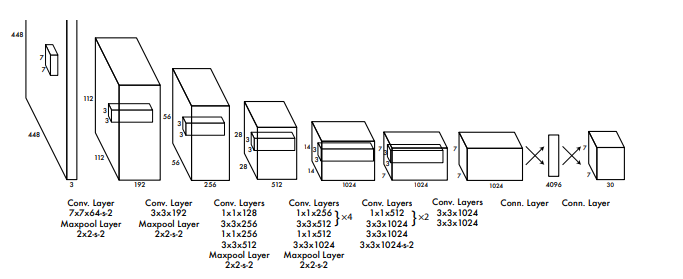
\includegraphics[width=0.9\textwidth,height=0.9\textheight,keepaspectratio]{imagenes/parte_IA/YOLOv1-architecture.png}    
    \caption{Arquitectura de la ``columna vertebral'' de YOLOv1.}
    \label{fig:yoloconvolutionlayers}
\end{figure}

\begin{figure}[]
    \centering
    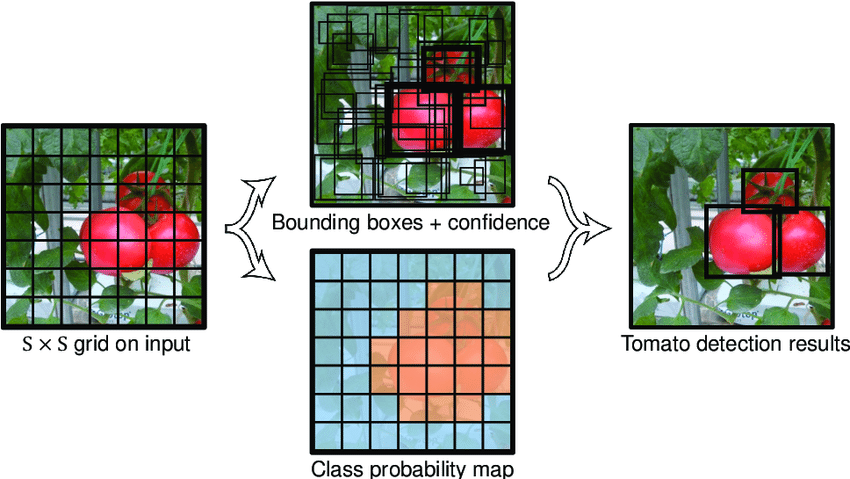
\includegraphics[width=0.78\textwidth,height=0.78\textheight,keepaspectratio]{imagenes/parte_IA/YOLO-simplify-steps.png}    
    \caption{Esquema del funcionamiento básico de YOLO.}
    \label{fig:yolosimplify}
\end{figure}

El funcionamiento de YOLO se muestra de forma simplificada en la figura \ref{fig:yolosimplify}. La cuarta versión \cite{yolov4originalpaper} se describe de forma general a continuación.

\begin{itemize}
    \item Primero se divide la imagen de entrada en cuadrículas de tamaño PxP píxeles. Cada cuadrícula será la responsable de detectar y localizar los objetos cuyo centro se encuentren en ella. El número de objetos que se pueden detectar por celdas varía en función de la versión utilizada; en la primera versión sólo se podía detectar un único objeto por celda, pero este valor ha ido aumentando en las versiones sucesivas.
    \item Tras dividir la imagen, esta se pasa por la red neuronal convolucional. Como resultado, en cada una de las celdas se predice un número B de objetos, estando representado cada objeto por un vector de 5+C elementos, donde C es el número de clases de objetos que podemos distinguir. Dicho vector tendrá la forma \\ $\rvect{P_c,B_x, B_y,B_w,B_h,C_1,C_2,...}$, donde:
    \begin{itemize}
        \item $P_c$ hace referencia a la confianza con la que se realiza la predicción de un objeto. Equivale al valor del índice de Jaccard entre la bounding box predicha y la supuesta bounding box real. Un valor de 0 indica que no se ha detectado ningún objeto, mientras que un valor 1 indica que se está completamente seguro de que hay un objeto contenido exactamente por la bounding box predicha.
        \item $B_x, B_y, B_w, B_h$ indican la posición X e Y del centro de la bounding box, así como el ancho y el alto de la misma. Los valores no se indican en unidades absolutas, como píxeles, si no que son proporcionales al ancho y alto de la celda.
        \item $C_0, C_1, ...$ indican si el objeto detectado corresponde a la clase de objeto con etiqueta 0, etiqueta 1, etc. Sólo uno de estos valores será 1, siendo el resto 0, ya que un objeto sólo puede pertenecer a una única clase.
    \end{itemize}
    Téngase en cuenta que si $P_c = 0$, el resto de valores del vector pueden ser ignorados, al no haberse detectado objeto alguno.
    \item Los cálculos anteriores generan multitud de predicciones duplicadas. Esto se debe a que varias celdas pueden haber detectado el mismo objeto, pero con bounding boxes diferentes. Por tanto, se debe utilizar algún mecanismo que nos permita seleccionar la mejor bounding box para cada objeto, descartando el resto. En particular, YOLO utiliza la técnica de la ``supresión de no máximos''.  
    \item La técnica de la ``supresión de los no máximos'' selecciona la bounding box con el valor $P_c$ (confianza en la predicción) más alto para cada etiqueta de clase y elimina las bounding boxes con la misma etiqueta de clase que se superpongan mucho con la caja seleccionada inicialmente. Normalmente se considera que las cajas se superponen mucho si se tiene un valor del índice de Jaccard igual o superior a 0.5. Este procedimiento se repite hasta que no se pueda eliminar ninguna bounding box más. En la figura \ref{fig:yolonmsexample} se puede apreciar la aplicación de este procedimiento, de manera que se obtiene como resultado una única bounding box para cada objeto, en este caso, de clases distintas. 
    \item Como resultado del proceso anterior, se retorna un vector de 6 elementos por cada objeto detectado. Los 5 primeros elementos coinciden con los del vector mostrado en puntos anteriores, siendo el sexto elemento el número de la etiqueta de clase del objeto detectado. Por tanto, los vectores resultantes tienen la forma $\rvect{P_c,B_x, B_y,B_w,B_h,C_N}$ 
\end{itemize}

\begin{figure}[]
    \centering
    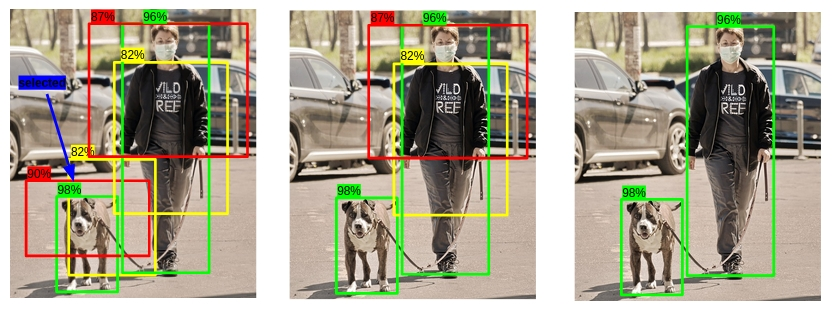
\includegraphics[width=0.9\textwidth,height=0.9\textheight,keepaspectratio]{imagenes/parte_IA/nms_yolo.jpg}    
    \caption{Aplicación de la supresión de no máximos.}
    \label{fig:yolonmsexample}
\end{figure}

Tras conocer el modus-operandi del detector de objetos YOLO, en la siguiente sección se explicarán los detalles del entrenamiento que se ha realizado para que este sea capaz de reconocer nadadores.

\section{Entrenamiento del modelo YOLOv4 para la detección de nadadores} 

En esta sección se detalla el proceso que se ha llevado a cabo para entrenar el modelo YOLOv4 de manera que sea capaz de detectar a los nadadores.

La primera decisión que se abordó fue si entrenar la red neuronal desde cero o utilizar los resultados de algún entrenamiento disponible en Internet y realizar un ajuste de manera que la red se especializara en la detección de nadadores.

Se optó por la segunda opción. Utilizamos un fichero de pesos resultado de haber entrenado la red en el conjunto de datos de prueba COCO (Common Objects in Context) \cite{cocodataset}. Esta base de datos está compuesta por unas 328.000 imágenes, entre las que se pueden reconocer 2.5 millones de objetos de 80 categorías distintas. Sin embargo, lo que hace esta base de datos especialmente adecuada para nuestra tarea es que tiene etiquetadas unas 250.000 personas. Así, la red neuronal ya posee de partida la capacidad de reconocer personas en multitud de situaciones. 

Sin embargo, este entrenamiento previo no es suficiente para conseguir detectar nadadores. Esto se debe principalmente a dos factores:
\begin{itemize}
    \item Las personas con las que ha sido entrenada la red siempre se encuentran en posición vertical, a diferencia de los nadadores, que se mueven a lo largo del eje horizontal de la piscina.
    \item En el conjunto de entrenamiento hay personas sin camiseta, con pantalones cortos (e incluso pañales), de espaldas, etc. Sin embargo, no hay apenas imágenes en las que haya personas en un ambiente en el que el agua es la componente principal, y además existan reflejos y cambios notables en la iluminación.
\end{itemize}
El primero de los problemas tiene fácil solución, rotar la imagen antes de hacer que la red neuronal la procese, de manera que el nadador estaría en vertical. Por desgracia, el segundo problema hace que la red no sea capaz de detectar a los nadadores en la gran mayoría de ocasiones.

Para solventar este inconveniente se hará uso de la técnica conocida como ``fine tuning''. Esta técnica consiste en, dada una red pre-entrenada en una base de datos distinta a la que se va a utilizar, realizar un pequeño segundo entrenamiento para mover el óptimo de la red hacia el óptimo de nuestro problema \cite{cnnindetail}. Esto nos permite enseñarle a la red a realizar una segunda tarea, en este caso el reconocimiento de nadadores, similar a la tarea en la que fue inicialmente entrenada, el reconocimiento de personas (entre otros objetos). Este enfoque nos permite reducir el tiempo de entrenamiento considerablemente, así como el número de imágenes de muestras necesarias para conseguir una correcta generalización y aprendizaje. 

El conjunto de imágenes utilizadas para el entrenamiento ha sido proporcionado por investigadores de la Facultad de Ciencias del Deporte de la UGR. El dataset consta de 1970 imágenes de resolución 120x120 píxeles en las que un nadador en posición vertical ocupa la mayor parte de cada imagen. Para cada una de estas imágenes se tiene un fichero de texto plano en el que se encuentra la etiqueta correspondiente en formato YOLO (numero de clase, coordenadas X e Y del centro de la bounding box, ancho y alto de la bounding box). En el conjunto de imágenes se tienen nadadores practicando diferentes estilos, así como momentos en los que los brazos del nadador están acoplados al cuerpo y momentos en los que se está realizando la voltereta con la que cambiar el sentido de nado al final de un split. 

Además, durante el entrenamiento se aplican técnicas de aumento de datos, entre las que se encuentran variaciones de la saturación, exposición y color de la imagen, redimensiones y recortes de la imagen, añadido de ruido gaussiano, etcétera. 

El software necesario para ejecutar YOLOv4 puede descargarse desde el repositorio oficial del autor \cite{darknetgithub}, Alexey Bochkovski. Para realizar la configuración seguiremos el manual que se proporciona y aplicaremos algunos consejos que se proporcionan en la sección wiki.

Los pasos seguidos para realizar el entrenamiento del modelo han sido los siguientes:

\begin{enumerate}
    \item Modificar los ficheros de configuración que serán utilizados para el entrenamiento. Primero, se crea una copia del fichero \textit{yolov4-custom.cfg}, ubicada en el directorio \textit{cfg}. Para este fichero, que se usará durante el entrenamiento, se realizan los siguientes cambios:
    
    \begin{itemize}
        \item \textit{Batch=32} y \textit{subdivisions=32}. El primer parámetro indica el número de imágenes que serán procesadas en un lote, mientras que el segundo se utiliza para calcular el número de mini lotes que serán procesados en paralelo por la GPU. Este valor será igual al resultado de dividir \textit{batch} y \textit{subdivisions}. Los valores de estos parámetros deben ser ajustados en función de la memoria de la que disponga la GPU. El autor recomienda mantener \textit{batch=64} siempre que se utilice una única tarjeta gráfica y modificar sólo el valor \textit{subdivisions}. Con la tarjeta gráfica de la que se disponía, NVIDIA GeForce GTX 1080, sólo se podían emplear combinaciones que tuvieran ambos valores iguales, en caso contrario se generaba un error por falta de memoria en la GPU. Se probó con valores iguales a 32 y 64, obteniendo resultados ligeramente mejores con 32.
        \item \textit{Width=416} y \textit{height=416}. Estos son el ancho y alto a los que se redimensionarán las imágenes al entrar a la red neuronal. Cuanto mayor sea este valor, mejor será el aprendizaje de la red. El autor recomienda cambiarlo a 608x608 o valores múltiplos de 32 superiores de ser posible. Sin embargo, cambiar el tamaño a 608x608 multiplicaba por cuatro el tiempo de entrenamiento, de manera que este podía llegar a alcanzar las 60 horas según las estimaciones realizadas por el propio software. Se tuvo que descartar al no ser asumible.
        \item \textit{Max\_batches=6000}. Este valor indica el número de iteraciones que tendrá el entrenamiento. Se recomienda asignar el resultado de multiplicar el número de tipos de objetos distintos que queramos detectar por 2000. En cualquier caso, el valor no debe ser inferior al número de imágenes de entrenamiento ni a 6000. Dado que solo teníamos una clase de objetos y 1970 imágenes, se asigno el valor 6000.
        \item \textit{Steps=4800,5400}. Este parámetro debe tener los valores correspondientes al 80 y 90\% del valor \textit{Max\_batches}.
        \item Para la última capa convolucional antes de cada una de las tres capas marcada como [yolo], deberemos cambiar el número de filtros por un valor tal que $filters=(classes+5)*3$. Por lo tanto, dado que sólo buscamos reconocer un tipo de objeto, se debe asignar \textit{filters=18} en las líneas 963, 1051 y 1139. Las capas marcadas como [yolo] son aquellas donde se realiza la detección de objetos. Cada una de ellas lo hace a diferente escala, de manera que se pueden detectar objetos de distinto tamaño.
        \item En las capas marcadas como [yolo] deberemos cambiar el parámetro \textit{classes} para que sea igual al número de tipos de objetos distintos que queramos distinguir. Por lo tanto, se debe asignar \textit{classes=1} en las líneas 970, 1058 y 1146. Nótese que aunque hay que reconocer una sola clase, el problema no es trivial, puesto que hay que ajustar las coordenadas de la bounding box que enmarcan al nadador. 
    \end{itemize} 
    
    A la hora de realizar la detección, deberemos crear un objeto de la clase \textit{dnn\_DetectionModel} de \textit{OpenCV}. Este constructor necesitará el fichero de configuración utilizado a la hora de entrenar y el fichero de pesos obtenido como resultado. En el código \textit{Python} se deberá establecer el tamaño al que se redimensionarán las imágenes antes de entrar a la red. Discutiremos la influencia de este parámetro en la sección \ref{evaluacionexpyolo}.
    
    \item Cargamos el conjunto de imágenes de entrenamiento, así como los ficheros de texto con las etiquetas, en el directorio \textit{data/obj}.
    
    \item Se deben crear dos ficheros de texto, \textit{data/train.txt} y \textit{data/valid.txt}, que contendrán las rutas a las imágenes que se utilizarán para el conjunto de entrenamiento y el conjunto de validación, respectivamente. Para realizar esta tarea se ha preparado un pequeño script que asigna el 85\% de las imágenes al conjunto de entrenamiento y el 15\% restante al conjunto de validación.
    
    \item Se debe crear el fichero \textit{data/obj.names}. Este contendrá los nombres de cada uno de los tipos de objetos a reconocer, uno por fila. Para este problema, sólo contendrá el valor ``person''. Debe tenerse cuidado y listar los nombres con el mismo orden que se utilizó al etiquetar los datos.
    
    \item Se tiene que crear el fichero \textit{data/obj.data}. Este contendrá el número de clases que queremos detectar, las rutas a los ficheros \textit{data/train.txt}, \textit{data/test.txt} y \textit{data/obj.names}, y la ruta al directorio donde guardaremos los ficheros generados como resultado del entrenamiento.
    
    \item También deberemos modificar las primeras líneas del fichero \textit{Makefile} para permitir el uso de la GPU, \textit{OpenCV} y \textit{CUDNN} (una librería para redes neuronales desarrollada por NVIDIA). En caso de disponer de una tarjeta gráfica con los llamados ``tensor cores'', habilitar el parámetro \textit{CUDNN\_HALF} permite reducir el tiempo de entrenamiento y detección considerablemente, en función de la resolución utilizada entre 2 y 4.5 veces \cite{darknetgithub}. Para habilitar estas opciones simplemente cambiaremos el valor 0 por el valor 1. Una vez se hayan realizado las modificaciones, se ejecutará el comando \textit{make} para generar el fichero ejecutable.
    
    \item Se debe descargar el fichero con los pesos resultantes de entrenar la red con el dataset COCO. Este fichero tiene como nombre \textit{yolov4.conv.137} y se puede encontrar en las publicaciones del repositorio \cite{darknetgithub}.
    
    \item Una vez se ha preparado todo lo necesario, deberemos ejecutar \textit{./darknet detector train data/obj.data cfg/yolov4-custom.cfg ../yolov4.conv.137 -dont\_show -map} para iniciar el entrenamiento de la red neuronal. 
\end{enumerate}

El primer entrenamiento del modelo que realizamos duró unas 7 horas y media aproximadamente. El software, al finalizar, mostraba por pantalla que se había alcanzado una precisión y recall de 1, es decir, todos los casos positivos habían sido clasificados correctamente. Esto es lógico dado que todas las detecciones realizadas corresponderían a la única clase que habíamos especificado. El valor medio del índice de Jaccard para predicciones realizadas con una confianza mínima del 25\% (mAP@0.25) era de 0.89, por lo que se había alcanzado un nivel de acierto en las predicciones muy alto. Los resultados obtenidos eran ciertamente prometedores.

Con este primer modelo, se realizó el primer intento de detección de nadadores para cada fotograma de un video. Sin embargo, a pesar de las métricas tan prometedoras obtenidas durante el entrenamiento, el modelo no era capaz de ubicar al nadador en ningún momento.

Analizando los resultados, el motivo es bastante directo. La red redimensiona las imágenes a su entrada, por tanto, cuando las imágenes de entrenamiento, de resolución 120x120 píxeles se redimensionan a un tamaño de 416x416 píxeles se mantiene la relación de aspecto, siguen siendo cuadradas, y el nadador no sufre ningún cambio. Sin embargo, los fotogramas de vídeo donde necesitamos detectar al nadador contienen una calle completa de la piscina, y tienen una resolución 120x1292 (relación 10.77:1). Redimensionar a un tamaño cuadrado, provoca que se deforme notablemente la figura del nadador, la cual no coincidirá con los ejemplos en los que la red neuronal se entrenó y hará que no se detecte nunca a dicho nadador. Esto se puede observar muy claramente en la figura \ref{fig:ejemplomalredimension}.

\begin{figure}
    \centering
    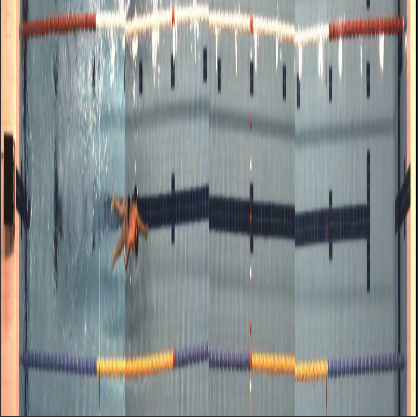
\includegraphics[width=0.5\textwidth,height=0.5\textheight,keepaspectratio]{imagenes/parte_IA/416x416_YOLO_resize.png}
    \caption{Redimensión de una calle de la piscina a tamaño cuadrado.}
    \label{fig:ejemplomalredimension}
\end{figure}

Para conseguir detectar a los nadadores se modificó el tamaño al que la red neuronal redimensiona los fotogramas del vídeo antes de procesarlos, con el objetivo de evitar que se modifique en exceso la apariencia del nadador. De esta manera, se consiguió que la red detectara a los nadadores a lo largo de la calle. Se han utilizado distintos tamaños de entrada, que se discuten en detalle en la sección \ref{evaluacionexpyolo}.

El siguiente problema apareció cuando los nadadores realizaban el giro y empezaban a nadar en sentido contrario. A partir de este momento, el nadador dejaba de ser detectado. La razón es que todos los datos de entrenamiento corresponden a nadadores en un único sentido. Esto afecta a la capacidad de detección de la red, que es incapaz de detectar a los nadadores que nadan en sentido contrario. 

Para solucionar este problema, se incluyó el volteo vertical entre las técnicas de aumento de datos, generando de esta forma las imágenes necesarias para detectar nadadores en el sentido contrario. 

Con esta nueva configuración, se realizó un nuevo entrenamiento de la red neuronal, el cual duró unas 16 horas aproximadamente. Tras este segundo entrenamiento, la red neuronal sí fue capaz de detectar a los nadadores a lo largo de todo el vídeo, independientemente del sentido del nado. Se obtuvo un valor de la precisión, recall e índice de Sorensen-Dice de 1, como era de esperar. Curiosamente, el valor medio del índice de Jaccard  para detecciones realizadas con un mínimo del 25\% de confianza (mAP@0.25) fue de 0.8432, algo menor que en el primer entrenamiento. 

Tras conseguir entrenar el modelo para realizar la detección de nadadores, en el siguiente apartado analizaremos la bondad de las predicciones y las compararemos con las realizadas por el modelo propuesto en el capítulo \ref{cap:capitulo3}.

\section{Evaluación experimental} \label{evaluacionexpyolo}

Con el objetivo de disponer de información que nos permita evaluar cuantitativamente los resultados, se han utilizado los mismos 45 fotogramas que se seleccionaron en el capítulo \ref{cap:capitulo3}. Así, se podrá también comparar los resultados proporcionados por este modelo y el propuesto en dicho capítulo.

En primer lugar, y como adelantábamos en la sección anterior, analizaremos la influencia del tamaño al que la red redimensiona las imágenes de entrada a la hora de realizar la detección de objetos. En la tabla \ref{tab:yolosizematters} se muestran los valores de los índices de Jaccard y Sorensen-Dice al utilizar diferentes valores de los parámetros (en píxeles), así como la confianza media con la que se realizan las predicciones. Además, se adjunta el tiempo de procesamiento medio (en milisegundos) por fotograma y la relación de aspecto para cada caso. 

\begin{table}
    \centering
    \small
    \begin{tabular}{| c | c | c | c | c | c | c| } \hline
        Ancho & Alto & IoU & F1-Score & Confianza & T.ejec (ms) & R.Aspecto \\ \hline
        416 & 416 & 0.00000 & 0.00000 & 0.000 & 19.141 & 1:1 \\
        416 & 4480 & 0.67197 & 0.80132 & \textbf{0.968} & 140.805 & 10.77:1* \\ 
        256 & 2688 & 0.72532 & 0.82767 & 0.818 & \textbf{54.571} & 10.5:1 \\ 
        416 & 2112 & \textbf{0.73378} & \textbf{0.84287} & 0.907 & 67.488 & 5.077:1  \\
        416 & 2528 & 0.71667 & 0.83191 & 0.945 & 78.505 & 6.077:1 \\ 
        416 & 3232 & 0.70861 & 0.82610 &  0.963 & 103.808 & 7.77:1 \\ \hline
    \end{tabular}
    \caption{Métricas en función de la redimensión realizada por la red. La relación de aspecto original aparece marcada con *.}
    \label{tab:yolosizematters}
\end{table}

En la primera prueba se mantuvieron los parámetros utilizados durante el entrenamiento. Así, las imágenes de la calle de la piscina donde se quiere realizar la detección, mucho más altas que anchas, se redimensionaban a un tamaño cuadrado de 416x416 píxeles. Como se explicó anteriormente, la variación de aspecto del nadador provoca que no se realice ninguna detección. Esto se puede observar en la primera fila de la tabla \ref{tab:yolosizematters}, en las que se puede apreciar valores del índice de Jaccard y Sorensen-Dice de 0.

Posteriormente, se utilizaron tamaños en los que se respeta la relación de aspecto de la imagen sobre la que se desea realizar la detección del nadador. De esta manera, el nadador no sufriría ninguna deformación, por lo que su aspecto sería idéntico al usado en las imágenes de entrenamiento pero con un tamaño mayor. Como se puede observar en la segunda y tercera fila de la tabla \ref{tab:yolosizematters}, las detecciones realizaron fueron bastante buenas al tener estas valores del índice de Jaccard y Sorensen-Dice superiores a 0.65 y 0.8, respectivamente. Inicialmente se probó un alto de 416 píxeles, mínimo recomendado por el autor, pero los tiempos eran demasiado altos, por lo que se probó a utilizar una resolución algo menor, con la que se consiguió no solo un tiempo de ejecución mucho menor, sino mejores resultados.

Finalmente, se probó a utilizar valores tales que las imágenes redimensionadas no mantuvieran la relación de aspecto, pero de manera que su alto fuera algo mayor que el alto original. En las tres últimas filas de la tabla \ref{tab:yolosizematters} se pueden apreciar los valores experimentales obtenidos para altos 1.63, 1.95 y 2.5 veces mayores que el original. Se eligieron estos valores dado que se mantiene el aspecto general del nadador, pero se dispone de un píxeles adicionales de alto, de manera que podría facilitarse la detección al ocupar el nadador un área algo mayor. Como se puede ver, los resultados obtenidos son ciertamente buenos. Para el caso de 416x2112 se obtuvieron los valores de las métricas utilizados más altos de todo el conjunto de experimentos de experimentos, incluso por encima de casos en los que sí se mantenía la relación de aspecto. Un ejemplo de cómo un fotograma con una calle se redimensiona a este tamaño se puede consultar en la figura \ref{fig:ejemplredimensiondoblealto}.

\begin{figure}
    \centering
    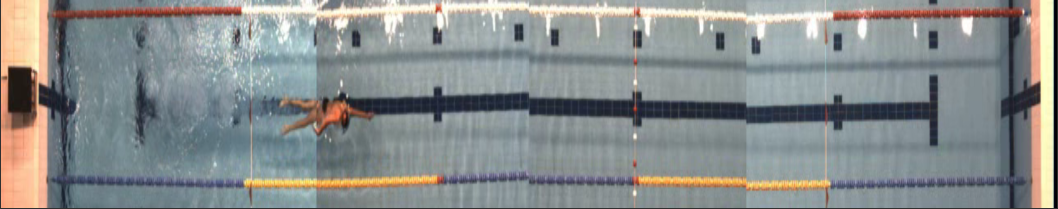
\includegraphics[width=\textwidth,height=\textheight,keepaspectratio]{imagenes/parte_IA/416x2112_YOLO_resize.png}
    \caption{Redimensión de una calle de la piscina para que tenga doble de alto.}
    \label{fig:ejemplredimensiondoblealto}
\end{figure}

Sin embargo, se decidió utilizar un tamaño de 256x2688 para redimensionar los fotogramas de los vídeos conforme entran a la red neuronal, dado que consideramos que es la combinación de valores que proporciona la mejor relación entre precisión en la predicción y tiempo de ejecución. Respecto del caso con dimensiones 416x2112 se obtuvieron valores del índice de Jaccard y Sorensen-Dice 0.001 y 0.015 menores, respectivamente. Esta pequeña diferencia no es prácticamente apreciable, ya que para valores del índice de Jaccard cercanos a 0.7 las predicciones son bastante buenas, pero gracias a ella se consigue una considerable mejora en el tiempo de ejecución del 19.14\%.

Tras evaluar el rendimiento del modelo basado en técnicas de aprendizaje profundo, compararemos el mismo con el modelo propuesto en el capítulo \ref{cap:capitulo3}. 

En la figura \ref{fig:iouvisualimgsyolo} se pueden observar seis fotogramas, que representan distintas condiciones de detección. Se remarcan en rojo las predicciones realizadas por el modelo basado en técnicas de aprendizaje profundo propuesto en este capítulo.

\begin{figure}[h!]
    \centering
    \begin{tabular}{cc}
          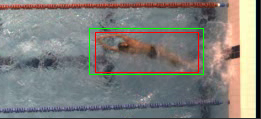
\includegraphics[width=0.43\textwidth,height=0.43\textheight,keepaspectratio]{imagenes/parte_IA/iou_visual/1099_recortada.png} &
          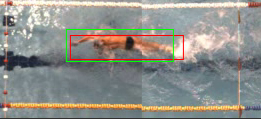
\includegraphics[width=0.43\textwidth,height=0.43\textheight,keepaspectratio]{imagenes/parte_IA/iou_visual/1259_recortada.png}
          \\ Fotograma A   & Fotograma B \\
          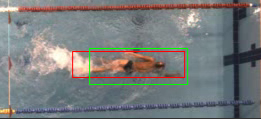
\includegraphics[width=0.43\textwidth,height=0.43\textheight,keepaspectratio]{imagenes/parte_IA/iou_visual/1014_recortada.png} &
          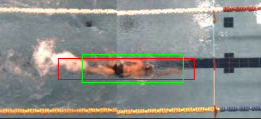
\includegraphics[width=0.43\textwidth,height=0.43\textheight,keepaspectratio]{imagenes/parte_IA/iou_visual/897_recortada.png}
          \\ Fotograma C & Fotograma D \\
          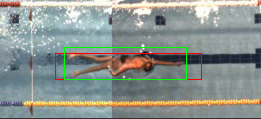
\includegraphics[width=0.43\textwidth,height=0.43\textheight,keepaspectratio]{imagenes/parte_IA/iou_visual/611_recortada.png} &
          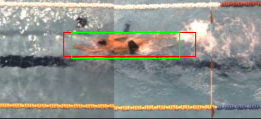
\includegraphics[width=0.43\textwidth,height=0.43\textheight,keepaspectratio]{imagenes/parte_IA/iou_visual/1241_recortada.png}
          \\Fotograma E & Fotograma F
     \end{tabular}
     \caption{Predicción automática (en rojo) frente a segmentación manual (en verde) para varios fotogramas.}
     \label{fig:iouvisualimgsyolo}
\end{figure}

\begin{table}[]
    \centering
    \begin{tabular}{| c | c | c | } \hline
        Fotograma & IoU & Sorensen-Dice \\ \hline
        A & 0.78566 & 0.87997  \\
        B & 0.67467 & 0.80574 \\   
        C & 0.62217 & 0.76708 \\ 
        D & 0.59528 & 0.74631 \\ 
        E & 0.70053 & 0.82390 \\ 
        F & 0.76596 & 0.86747 \\ \hline
    \end{tabular}
    \caption{Métricas para predicciones frente a segmentación manual para varios fotogramas.}
    \label{tab:iouvisualtabyolo}
\end{table}

Como se puede apreciar, YOLOv4 es capaz de identificar al nadador en su totalidad en todos los fotogramas, mientras que el enfoque del capítulo \ref{cap:capitulo3} genera predicciones en las que sólo se reconoce el tronco superior del nadador. También se puede observar cómo las predicciones de YOLO tienden a incluir parte del agua en la bounding box que contiene al nadador, aunque reducen considerablemente la cantidad de agua detectada como parte del nadador en fotogramas en los que existen un gran chapoteo.

En la tabla \ref{tab:iouvisualtabyolo} se pueden observar los valores de los índices de Jaccard y Sorensen-Dice para las predicciones presentadas en la figura \ref{fig:iouvisualimgsyolo}. Todos los fotogramas presentan un valor IoU superior a 0.6, a partir del cual podemos considerar las predicciones como acertadas, teniendo 4 de los 6 fotogramas un valor superior a 0.67. Si se comparan estos valores con los presentados en la tabla \ref{tab:iouvisualtab} para la aproximación del capítulo \ref{cap:capitulo3}, se observa una mejora sustancial para los tres primeros fotogramas y una ligera disminución de la precisión de la predicción para los dos últimos fotogramas.

Tras haber ejemplificado las diferencias entre los enfoques para seis fotogramas concretos, abordemos los resultados medios obtenidos para los 45 fotogramas utilizados en el conjunto de pruebas. En la tabla \ref{tab:metricasaproximaciones} se muestran los valores medios de los índices de Jaccard y Sorensen-Dice, así como el tiempo medio de procesamiento por fotograma para ambos enfoques. 

\begin{table}[]
    \centering
    \begin{tabular}{| c | c | c | c | } \hline
        Enfoque & IoU & F1Score  & T.ejecución (ms)  \\ \hline
        GSoC sobre Cr & 0.64126 & 0.76864 & \textbf{11.051} \\
        YOLOv4 & \textbf{0.72532} & \textbf{0.82767} & 54.571  \\ \hline
    \end{tabular}
    \caption{Métricas para cada aproximación.}
    \label{tab:metricasaproximaciones}
\end{table}

Como se podía intuir, YOLO obtiene métricas mejores que el modelo propuesto en el capítulo \ref{cap:capitulo3}. Esto se debe principalmente a dos factores:
\begin{enumerate}
    \item YOLO es capaz de detectar al nadador completo donde la aproximación del capítulo anterior sólo detecta modo el tronco del nadador.
    \item YOLO reduce en gran medida la cantidad de agua reconocida como parte del nadador en fotogramas donde existe un gran chapoteo, aunque tiende a incluir de manera general un poco de agua en las bounding box de las predicciones.
\end{enumerate}

En contraposición, el modelo basado en técnicas de aprendizaje profundo requiere de un tiempo de procesamiento considerable, dado que es 4.94 veces más lento que el enfoque propuesto en el capítulo \ref{cap:capitulo3}. 

Tras analizar el rendimiento del método basado en aprendizaje profundo, y compararlo con el rendimiento ofrecido por el modelo propuesto en el capítulo \ref{cap:capitulo3}, en el capítulo \ref{cap:capitulo5} se detallará el método que se utilizará para calcular la frecuencia media de nado y se decidirá que algoritmo de detección de objetos ofrece mejores resultados.

